%!TEX program = xelatex
%!TEX options = --shell-escape
\documentclass{beamer}

\input{_header}

\author{T. Hater}
\institute{Forschungszentrum J\"ulich}
\title{Get yourself (re)connected}
\subtitle{Structural Plasticity in Arbor\newline{}\small{Technical Background, Foundations, and Future Plans}}
\date{September 2022}

\input{_customizations}

\usetikzlibrary{shapes.geometric}

\titlegraphic{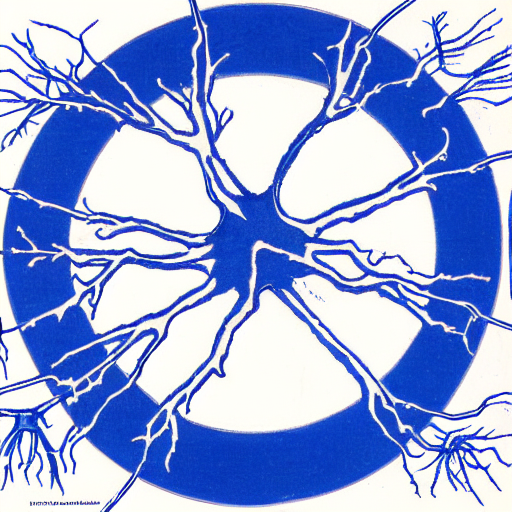
\includegraphics[width=\paperwidth]{images/neuron}}

\begin{document}
\maketitle

\begin{frame}{Topics}{abc}
  \begin{itemize}
    \item Technical background of Arbor's connectivity.
    \item Structural Plasticity in Arbor.
    \item Demo!
    \item Calcium tracking.
    \item Diffusion.
    \item Future Plans
          \begin{itemize}
            \item A DSL for connectivity.
            \item Dynamic matching.
            \item \dots
          \end{itemize}
  \end{itemize}
\end{frame}

\begin{frame}[fragile]{From Recipe to Network}{\dots and beyond}
\begin{codePythonblock}
import arbor as A

class Recipe(A.recipe):
    def connections_on(self, target_gid):
        return [A.connection((source_gid,   # cell from which spikes are coming in
                              "source"),    # label of the detector on that cell
                             "synapse",     # label of the synapse on our cell
                             weight,        # connection weight
                             delay),        # axonal + synaptic delay
                # ...
                ]
\end{codePythonblock}
\begin{itemize}
  \item \texttt{gid}s are unsigned numbers to label a cell
  \item \texttt{"label"}s are used to designate items on cells
  \item each cell may return different sources based on its own \texttt{gid}
  \item there are similar mechanisms for local generators and gap junctions
\end{itemize}
\end{frame}

\begin{frame}[fragile]{Transmission of Spikes}
  \begin{itemize}
    \item Communication pattern: collect all spikes on all receiving processes
          \begin{itemize}
            \item Spikes are sent as \verb!(source, weight, time)!
            \item These are locally sorted, \verb!AllGather!ed, and thus globally sorted!
            \item Receivers filter by 'their' sources (\verb!bsearch!)
          \end{itemize}
  \end{itemize}
  \begin{center}
    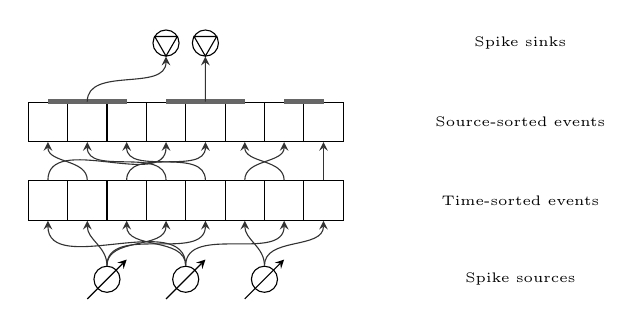
\begin{tikzpicture}
      \foreach \x in {0,...,2} \node[circle, draw, xshift=0.75cm] (det\x) at (\x,0) {};
      \foreach \x in {0,...,2} \draw[->, >=stealth, xshift=0.75cm] (\x-0.25,-0.25) -- (\x+0.25,0.25);
      \foreach \x in {0,...,7} \node[draw, rectangle, minimum width=5mm, minimum height=5mm] (evt\x) at (\x*5mm,1) {};
      \foreach \x in {0,...,7} \node[draw, rectangle, minimum width=5mm, minimum height=5mm] (sor\x) at (\x*5mm,2) {};
      \foreach \x in {0,...,1} \node[draw, circle, anchor=center, xshift=1.5cm] (syn\x) at (0.5*\x,3) {};
      \foreach \x in {0,...,1} \node[regular polygon, draw, regular polygon sides=3, scale=0.5, rotate=180, xshift=-3.0cm] at (0.5*\x,3) {};
      %
      \draw[->, >=stealth, black!80] (det0.north) to [in=270, out=90] (evt1.south);
      \draw[->, >=stealth, black!80] (det0.north) to [in=270, out=90] (evt3.south);
      \draw[->, >=stealth, black!80] (det0.north) to [in=270, out=90] (evt4.south);
      \draw[->, >=stealth, black!80] (det1.north) to [in=270, out=90] (evt0.south);
      \draw[->, >=stealth, black!80] (det1.north) to [in=270, out=90] (evt2.south);
      \draw[->, >=stealth, black!80] (det1.north) to [in=270, out=90] (evt6.south);
      \draw[->, >=stealth, black!80] (det2.north) to [in=270, out=90] (evt5.south);
      \draw[->, >=stealth, black!80] (det2.north) to [in=270, out=90] (evt7.south);
      %
      \draw[->, >=stealth, black!80] (evt1.north) to [in=270, out=90] (sor0.south);
      \draw[->, >=stealth, black!80] (evt3.north) to [in=270, out=90] (sor1.south);
      \draw[->, >=stealth, black!80] (evt4.north) to [in=270, out=90] (sor2.south);
      \draw[->, >=stealth, black!80] (evt0.north) to [in=270, out=90] (sor3.south);
      \draw[->, >=stealth, black!80] (evt2.north) to [in=270, out=90] (sor4.south);
      \draw[->, >=stealth, black!80] (evt6.north) to [in=270, out=90] (sor5.south);
      \draw[->, >=stealth, black!80] (evt5.north) to [in=270, out=90] (sor6.south);
      \draw[->, >=stealth, black!80] (evt7.north) to [in=270, out=90] (sor7.south);
      %
      \draw[black!60, ultra thick] (sor0.north) -- (sor2.north);
      \draw[black!60, ultra thick] (sor3.north) -- (sor5.north);
      \draw[black!60, ultra thick] (sor6.north) -- (sor7.north);
      %
      \draw[->, >=stealth, black!80] (sor1.north)  to [in=270, out=90] (syn0.south);
      \draw[->, >=stealth, black!80] (sor4.north)  to [in=270, out=90] (syn1.south);
      %
      \node at (6, 0) {\tiny{Spike sources}};
      \node at (6, 1) {\tiny{Time-sorted events}};
      \node at (6, 2) {\tiny{Source-sorted events}};
      \node at (6, 3) {\tiny{Spike sinks}};
    \end{tikzpicture}
  \end{center}
  \begin{itemize}
    \item Conncurrent communication and computation based on decoupling
          \begin{itemize}
            \item Pick the global minimum $\tau$ over \verb!delay!; half for double-buffering.
            \item No event at $t$ can influence anything before $t + \tau$
          \end{itemize}
  \end{itemize}
\end{frame}

\begin{frame}[fragile]{Local Filtering}{\dots and Plasticity}
  \begin{itemize}
    \item Each process holds a list of sources it's connected to; plus their associated targets.
    \item This table is built using the \verb!connections_on! data
    \item Thus, to modify the connections, we just need to tweak this table.
    \item However, it's simpler, safer, and faster to completely rebuild.
    \item This is a \emph{purely local}, independent process.
  \end{itemize}
\end{frame}

\begin{frame}[fragile]{Structural Plasticity}{Bare Bones Example}
\begin{codePythonblock}
  import arbor as A
  # contains initial network
  rec = my_recipe()
  # run the network for 5ms
  sim = A.simulation(rec)
  sim.run(5)
  # here we update the recipe, or create a new one
  rec = ...
  # rebuild connection table
  sim.update(rec)
  # ... and continue simulating
  sim.run(5)
\end{codePythonblock}
\begin{itemize}
  \item Add/delete synaptic connections and event generators and adjust their weights.
  \item \textcolor{red}{Not changed}: Gap Junctions, detectors, cells, parameters, morphology, and synapses.
\end{itemize}
\end{frame}

\begin{frame}{Demo!}
  \begin{center}
    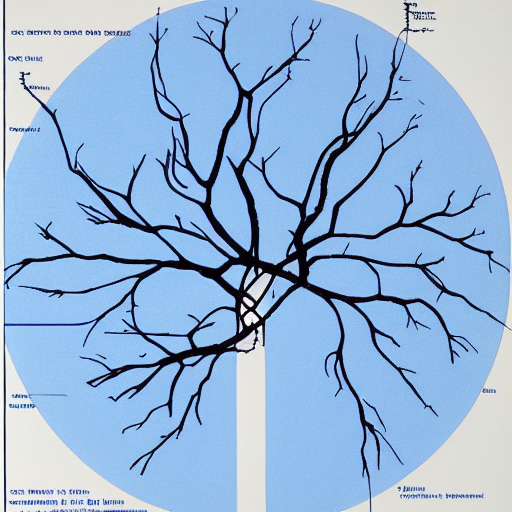
\includegraphics[width=0.5\textwidth]{images/neuron-2}
  \end{center}
\end{frame}

\begin{frame}[fragile]{Calcium Tracking}
  \begin{codePythonblock}
    class Recipe(A.recipe):
        # ...
        def probes_on(self, gid):
            if gid == 0:
                # Probe ca concentration on a given set of locations (here: all terminals)
                return [A.cable_probe_ion_int_concentration('(terminal)', 'ca')]
            elif gid == 42:
                # Probe ca on every cable in the cell
                return [A.cable_probe_ion_int_concentration_cell('ca')]
            else:
                return []

    rec = Recipe()
    sim = simulation(rec)
    hd0 = sim.sample((0, 0), A.regular_schedule(0.1))  # 1st probe on gid=0: terminals
    hd1 = sim.sample((42, 0), A.regular_schedule(0.1)) # 1st probe on gid=42: all cables
    sim.run(23)
    results = sim.samples(hd0)
    # ...
  \end{codePythonblock}
\end{frame}

\begin{frame}[fragile]{Diffusing Molecules}
  \begin{codePythonblock}
    tree = load_swc_arbor(...)
    labels = A.label_dict()
    decor = (A.decor()
          .set_ion("na", int_con=0.0, diff=0.005)                     # Add diffusion to Sodium
          .place("(location 0 0.5)", A.synapse("inject/x=na"), "Zap") # Synapse to produce Na
          .paint("(all)", A.density("decay/x=na")))                   # Na decays exponentially

    cell = A.cable_cell(tree, labels, decor)
  \end{codePythonblock}
  \begin{itemize}
    \item No longer part of the cable model, but separate!
    \begin{itemize}
      \item Breaks thin shell approximation,
      \item no reset like for internal/external concentration $ X_{i}$ and  $X_{o}$,
      \item $\partial_{t} X_{d}$ does not contribute to current (neither do $\partial_{t} X_{i}$ and $\partial_{t} X_{o}$).
    \end{itemize}
    \item Can be used as
    \begin{itemize}
      \item a memory mechanism,
      \item transmitter between spatial separated synapses.
    \end{itemize}
    \item Can be probed just like  $ X_{i}$ and  $X_{o}$.
  \end{itemize}
\end{frame}

\begin{frame}{Future Plans}
  \begin{center}
    \includegraphics[width=0.5\textwidth]{images/neuron-3}
  \end{center}
\end{frame}

\begin{frame}[fragile]{Connectivity}
  \begin{itemize}
    \item Currently connectivity is defined via lists of indices and labels.
    \item UX does not scale and is not ergonomic even at small scales.
    \item Thus: define a high-level connection DSL, loosely inspired by NMLlite.
  \end{itemize}
  \begin{codePythonblock}
  (connect
    (from                         ; sources
      (all)                       ; all gids
      (is-kind spike-detector))   ; source labels
    (to                           ; targets
      (distance-lt 0.42)          ; L2 distance src <-> tgt
      (is-kind 'expsyn')))        ; target labels
  \end{codePythonblock}
  \begin{itemize}
    \item Design is work in progress, phase space is huge.
    \item Probabilistic connectivity, tag based queries, relational algebra, \dots
  \end{itemize}
\end{frame}

\begin{frame}[fragile]{Selecting Target/Source Pairs}
  \begin{itemize}
    \item (Re)Connecting cells requires spatial queries across multiple ranks in
          a parallel computation.
    \item Investigate algorithms for finding partners, starting simple.
    \item More scalable approaches like Rinke et al '17 might be interesting.
  \end{itemize}
\end{frame}

\begin{frame}[fragile]{Possible Explorations}
  \begin{itemize}
    \item Modifying parameters during simulation.
    \item Tweaking the morphology.
    \item Re-connecting Gap Junctions (when we have implemented a distributed
          algorithm)
  \end{itemize}
  \begin{block}{Disclaimer}
    These are hard(er) problems and might not be feasible to implement.
  \end{block}
\end{frame}

\begin{frame}
  \frametitle{Summary}
  \begin{itemize}
    \item Plasticity is an active driver for Arbor development.
    \item We already have solid foundations in place.
    \item From here, your input is needed.
  \end{itemize}
  \begin{tikzpicture}[overlay, remember picture]
    \node<2-> [draw=fzjblue50, fill=fzjblue50!3, inner sep=5pt, outer sep=4pt, anchor=south east, font=\bfseries\larger\itshape, align=center, text=fzjblue50, rotate=8] at ([yshift=60pt,xshift=-40]current page.south east) {
      Thank you!\\[-0.3ex]Questions?\\{\relsize{-3}\href{mailto:t.hater@fz-juelich.de}{t.hater@fz-juelich.de}}
    };
  \end{tikzpicture}
\end{frame}

\end{document}
